\chapter{Despliegue} \label{despliegue}

En este capítulo se va a proceder a explicar los pasos seguidos para realizar el despliegue en la nube de la aplicación. Para ello se han utilizado dos plataformas diferentes: \textbf{Github Pages}, que ha permitido desplegar el frontend y \textbf{Railway} \cite{Railway} dónde se han desplegado los 5 microservicios, las tres bases de datos PostgreSQL y un servicio de RabbitMQ. A continuación, se va a mostrar cómo se han realizado ambos despliegues.

\section{Despliegue del frontend}
\begin{figure}[H]
  \centering
  
\includegraphics[width=0.6\textwidth]{fotos/pages.jpg}
  \caption{Logo Github Pages}
  \label{fig:pages}
\end{figure}
Para el despliegue del frontend se ha utilizado la plataforma \textbf{GitHub Pages}, una herramienta gratuita que ofrece GitHub para desplegar sitios estáticos. En nuestro caso, se trata de un proyecto React compilado. 

El procedimiento seguido consiste en:

\begin{enumerate}
    \item Instalar en el proyecto React la dependencia \texttt{gh-pages} mediante el comando:
    \begin{verbatim}
    npm install --save-dev gh-pages
    \end{verbatim}
    
    \item Configurar la variable \texttt{homepage} en el archivo \texttt{package.json} para indicar la URL de despliegue.
    
    \item Ejecutar el comando:
    \begin{verbatim}
    npm run deploy
    \end{verbatim}
\end{enumerate}

Para integrar este proceso dentro del flujo de desarrollo de la aplicación, el frontend se ha desplegado automáticamente cada vez que se realizaba un \textbf{merge} a la rama \texttt{main} (equivalente a producción), gracias a una acción específica configurada en \textbf{GitHub Actions}. 

Finalmente, para que el frontend pueda realizar las llamadas correspondientes tanto en local como en producción, se han configurado una serie de archivos de entorno (\texttt{.env}) que determinan la ruta de consulta correcta en cada caso.

\vspace{0.25em}
Enlace al frontend desplegado: \href{https://alonsodm12.github.io/TFG_COHOUSING/}{Share-Space}


\section{Despliegue del backend}

\begin{figure}[H]
  \centering
  
\includegraphics[width=1\textwidth]{fotos/railway.png}
  \caption{Logo Railway}
  \label{fig:railway}
\end{figure}
Para el despliegue del backend se ha utilizado Railway, un PaaS (Platform as a Service) en la nube que facilita el despliegue de servicios directamente desde repositorios de GitHub, Dockerfiles o plantillas de servicios.

Dentro de Railway se han definido dos proyectos independientes, imagen \ref{fig:railway1} e imagen \ref{fig:railway2}, en los que se han desplegado los distintos servicios que componen el sistema.

\begin{figure}[H]
  \centering
  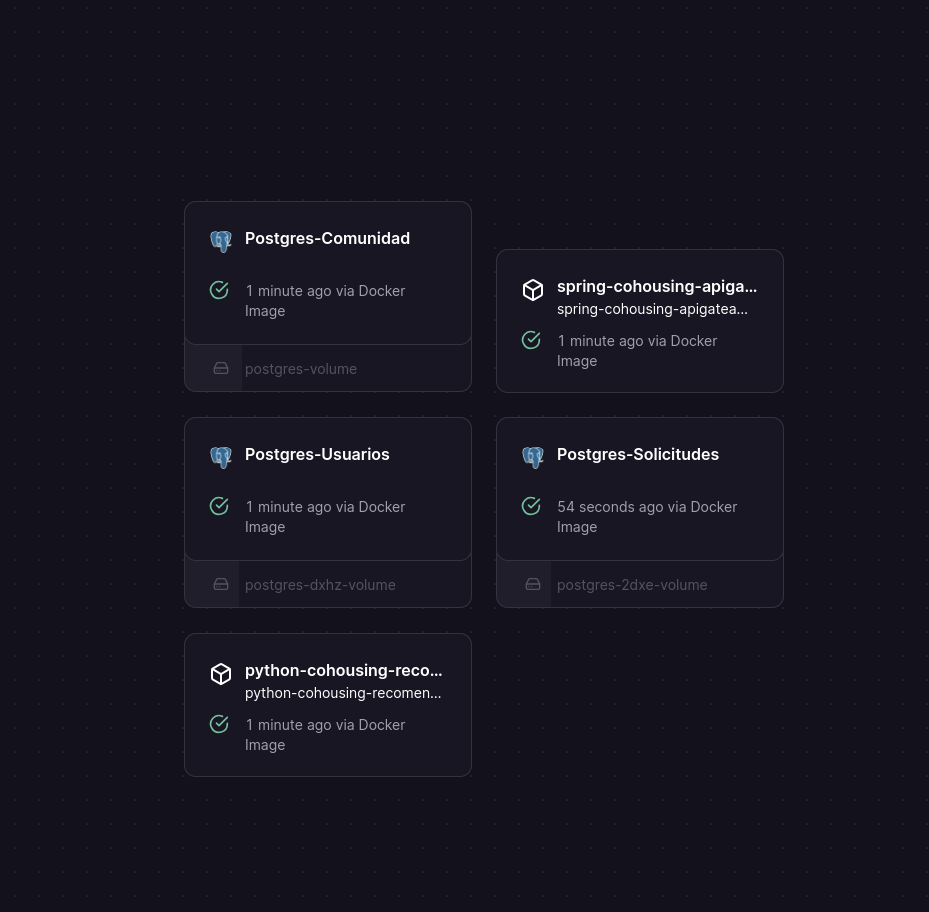
\includegraphics[width=1\textwidth]{fotos/railway1.png}
  \caption{Muestra del tablero de despliegue del primer proyecto en Railway}
  \label{fig:railway1}
\end{figure}


\begin{figure}[H]
  \centering
  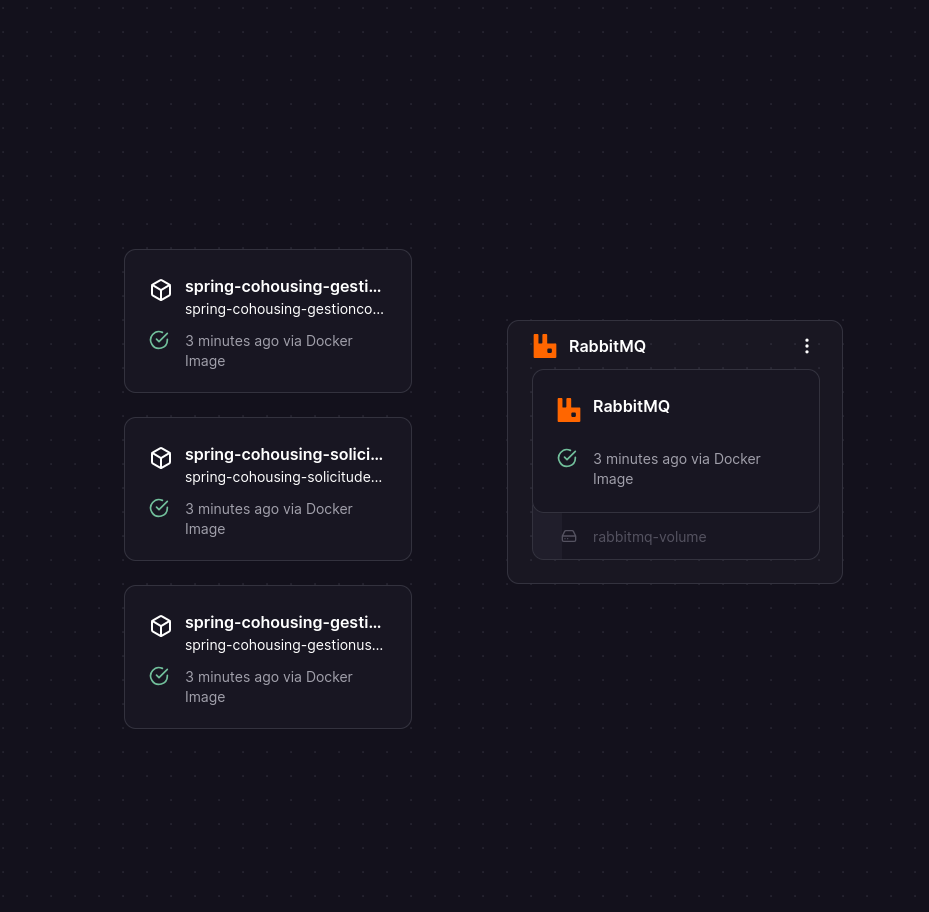
\includegraphics[width=1\textwidth]{fotos/railway2.png}
  \caption{Muestra del tablero de despliegue del segundo proyecto en Railway}
  \label{fig:railway2}
\end{figure}
Cada microservicio ha sido desplegado en \textbf{Railway} a partir de su respectivo Dockerfile subido a DockerHub, estos han ido actualizándose cada vez que se realizaba un \textbf{merge} a la rama \texttt{main} (producción). Además, se ha configurado una serie de variables para cada servicio, de forma que puedan conectarse con las bases de datos y con el servicio de RabbitMQ. Estas variables son inyectadas automáticamente en el código a partir de un archivo \texttt{application-prod.properties} y un perfil activo \texttt{prod}.

En cuanto a la seguridad, tanto Railway como GitHub Pages proporcionan URLs para cada servicio con \textbf{HTTPS}, lo que garantiza que el tráfico entre el cliente y los servicios esté cifrado, evitando el envío en texto plano.

\vspace{0.5em}
Los servicios desplegados en Railway han sido los siguientes:
\vspace{0.5em}
\begin{itemize}
    \item \textbf{Microservicio de Gestión de Usuarios}: \url{https://spring-cohousing-GestionUsuarios-production.up.railway.app} \vspace{0.5em}
    \item \textbf{Microservicio de Gestión de Comunidades}: \url{https://spring-cohousing-GestionComunidades-production.up.railway.app} \vspace{0.25em}
    \item \textbf{Microservicio Recomendador}: \url{https://python-cohousing-recomendador-production.up.railway.app} \vspace{0.25em}
    \item \textbf{Microservicio de Solicitudes}: \url{https://spring-cohousing-Solicitudes-production.up.railway.app} \vspace{0.25em}
    \item \textbf{Bases de datos}: Tres bases de datos PostgreSQL denominadas \texttt{Postgres} 
    \texttt{-Comunidad}, \texttt{Postgres-Usuarios} y \texttt{Postgres-Solicitudes} \vspace{0.25em}
    \item \textbf{Microservicio ApiGateway}: \url{https://spring-cohousing-apigateaway-production.up.railway.app} \vspace{0.25em}
    \item \textbf{Servicio RabbitMQ}: Desplegado a partir de una plantilla obtenida en DockerHub.
\end{itemize}

Finalmente,en la imagen \ref{fig:onboard}, mostramos la página de bienvenida del sistema, ya accesible desde la red.
\begin{figure}[H]
  \centering
  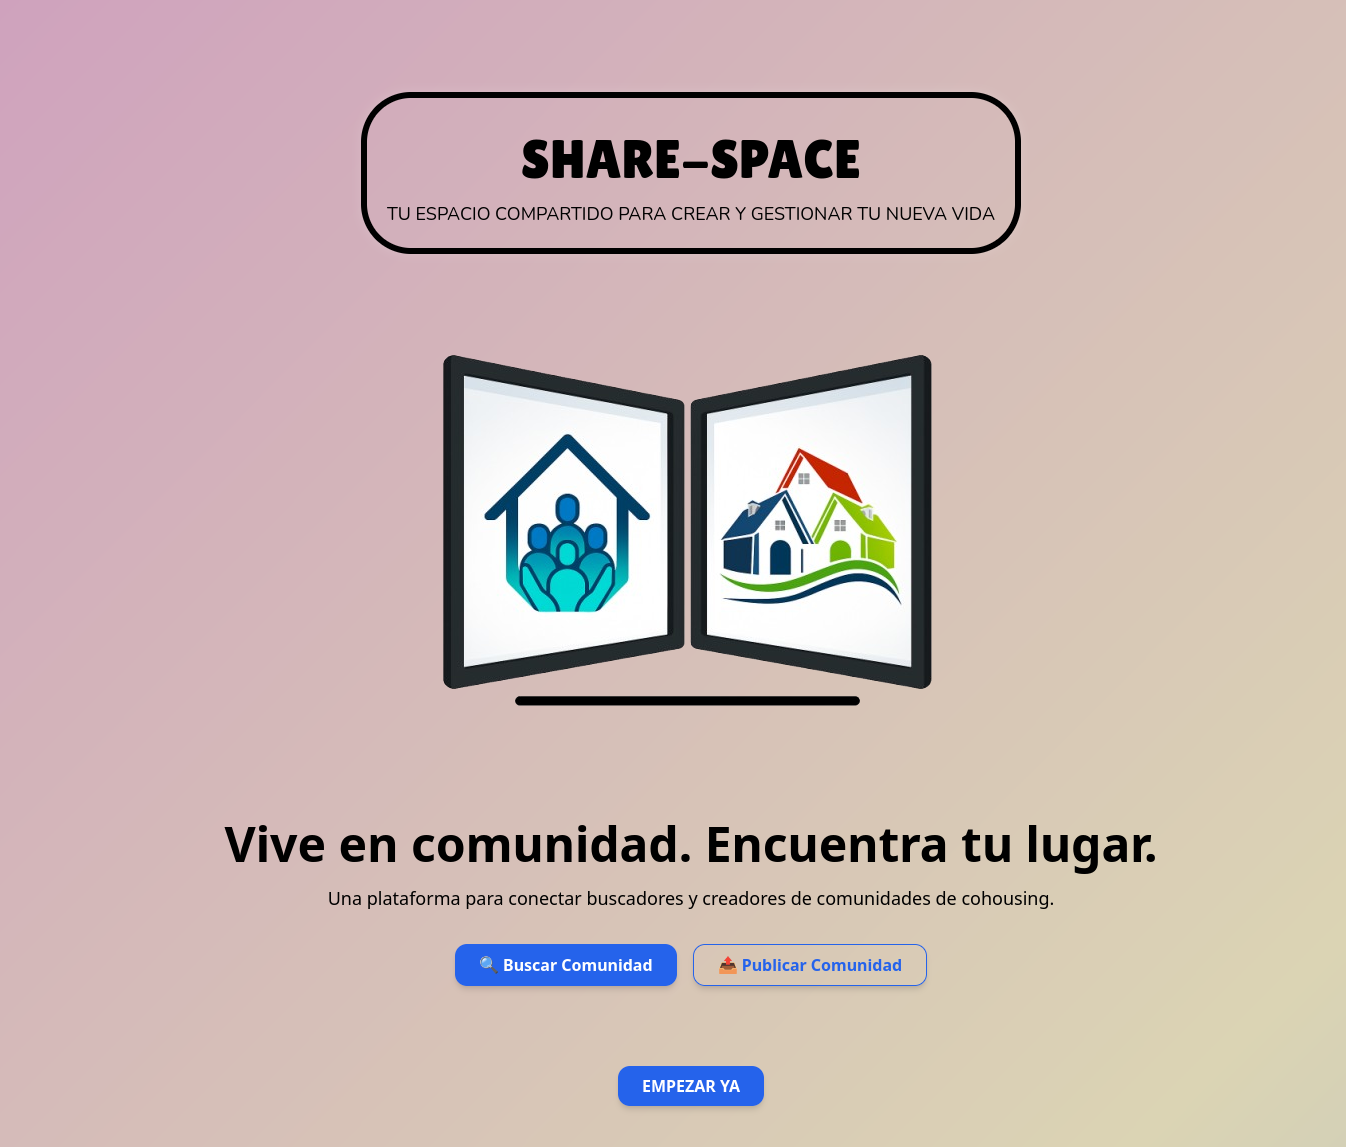
\includegraphics[width=1\textwidth]{fotos/onboard.png}
  \caption{Página de bienvenida del sistema}
  \label{fig:onboard}
\end{figure}

\vspace{0.5em}

